\documentclass[12pt]{article}

\usepackage{sbc-template}

\usepackage{graphicx,url}
\usepackage{subfigure}

%\usepackage[portuguese]{babel}   
\usepackage[utf8]{inputenc}  

\usepackage{listings}
\lstset{
  language=C++,
  basicstyle=\ttfamily\small, 
  keywordstyle=\color{blue}, 
  stringstyle=\color{verde}, 
  commentstyle=\color{red}, 
  extendedchars=true, 
  showspaces=false, 
  showstringspaces=false, 
  numbers=left,
  numberstyle=\tiny,
  breaklines=true, 
  backgroundcolor=\color{white!10},
  breakautoindent=true, 
  captionpos=b,
  xleftmargin=0pt,
}
     
\sloppy

\title{Microservicio web para la detección de rostros.\\Web microservice for face detection.}
\author{Chica Gòmez Ruth Estefania , Caza Romero Diana Paola.
}


\address{
UNIVERSIDAD LAICA ELOY ALFARO DE MANABI
\\
  ESTUDIANTES DE LA CARRERA TECNOLOGIAS DE LA INFORMACION\\
  SISTEMAS DISTRIBUIDOS\\
  EL Carmen – Ecuador
 \email{\{Chica Gòmez Ruth Estefania , Caza Romero Diana Paola\}@gmail.com}
}

\begin{document} 

\maketitle

\begin{resumo} 
  El proyecto investiga el reconocimiento de rostros, que es esencial para el reconocimiento humano, utilizando tecnología avanzada de inteligencia artificial y aprendizaje profundo. Utilizando FaceNet-PyTorch, crea un microservicio de reconocimiento de rostros que ofrece soluciones precisas, felxible y adaptables. El programa optimiza la gestión de datos y tiene el potencial de tener un impacto en una variedad de aplicaciones.\\
  \textbf{Palabras clave}: Detección, microservicios, reconocimiento, rasgos, rostros.
\end{resumo}
\begin{abstract}
  The project investigates face recognition, which is essential for human recognition, using advanced artificial intelligence and deep learning technology. Using FaceNet-PyTorch, create a face recognition microservice that delivers accurate, adaptive, and adaptive solutions. The program optimizes data management and has the potential to impact a variety of applications.\\
  \textbf{Keywords:} Detection, microservices, recognition, features, faces.
\end{abstract}

\section{Introducciòn}

El reconocimiento facial ha sido un componente crucial para la identificación interpersonal desde la civilización. El rostro humano es una manifestación intrínseca de la identidad individual y es sensible a los rasgos faciales. La inteligencia artificial y el aprendizaje profundo ha evolucionado desde métodos rudimentarios hasta algoritmos que minimiza los errores. Estos avances han expandido la aplicabilidad del reconocimiento facial más allá de la seguridad pública, en sectores como la banca, publicidad y atención sanitaria.\\
La arquitectura de microservicio fomenta el desarrollo de software al brindar escalabilidad, modularidad y eficiencia. El objetivo de esta investigación es superar las limitaciones de los métodos tradicionales mediante la creación de un microservicio de reconocimiento de rostros utilizando los algorithmos avanzados de FaceNet-PyTorch para la detección y comparación de rostros.
Este proyecto presenta un microservicio web diseñado para la detección de rostros utilizando la técnica de aprendizaje profundo FaceNet-PyTorch. El microservicio se enfoca en proporcionar una interfaz eficiente y robusta para la detección de rostros en tiempo real.
\begin{figure}
	    \centering
	    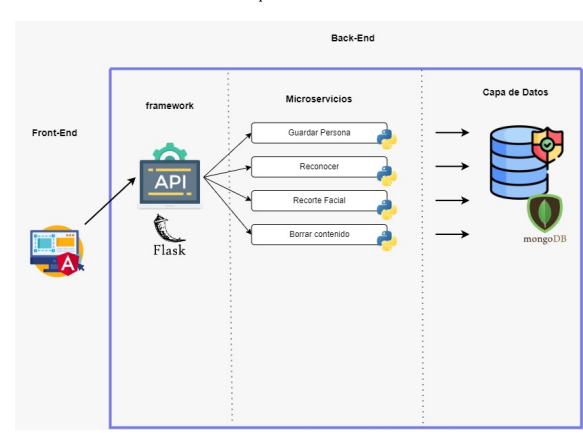
\includegraphics[width=0.6\linewidth]{image.png}
	    \caption{Arquitectura del Sistema}
	    \label{fig:enter-label}
	\end{figure}	

\section{Materiales y Métodos} \label{sec:firstpage}
La siguiente es una revisión del estado del arte en este campo, destacando las técnicas previamente utilizadas y describiendo las particularidades de la investigación actual.\\
Palomeque, Heras y Quevedo crearon un sistema para monitorear y prevenir accidentes laborales enfocado en el sector de la construcción. Este sistema analiza imágenes y videos de construcción con técnicas de Deep Learning y algoritmos YOLOv5(una herramienta de la inteligencia artificial que tiene un talento especial para reconocer objetos en imágenes y videos)el cual identifica áreas de interés y determinar si los empleados utilizan correctamente el equipo de protección personal.\\
Para reducir la trata de personas, Barreto Rodríguez propuso un sistema de reconocimiento facial. Su método se basa en OpenFace(Detecta puntos de referencia faciales, Estimación de la pose de la cabeza, Reconocimiento de unidades de acción faciales), un marco que combina tecnologías como Python, Torch y OpenCV y que ha demostrado un índice de acierto del 95porciento en tareas de detección facial.\\
La técnica de aprendizaje profundo FaceNet-PyTorch es fundamental para la detección de rostros en tiempo real.
Se utiliza un microservicio web para proporcionar una interfaz eficiente y accesible a las capacidades de detección de rostros.El framework Flask se utiliza para la construcción del backend del microservicio web, lo que facilita el desarrollo de la API.
Se utiliza un conjunto de datos de imágenes de rostros para entrenar el modelo de detección de rostros.
\section{Arquitectura} 
Este estudio diseñó una arquitectura de microservicio para capturar, procesar y identificar imágenes faciales utilizando un sistema de redes neuronales convolucionales y algoritmos de detección facial para comparar, buscar y reconocer rostros.
La arquitectura de servicio combina varias tecnologías para implementar microservicios, utilizando la interfaz de usuario dinámica y el marco de Flask(marco de desarrollo web de código abierto, escrito en Python). La API conecta estos servicios, sirviendo como intermediario para administrar solicitudes y respuestas. También se establece un límite de almacenamiento de datos para el desarrollo y operación eficientes de las aplicaciones.\\
El back-end está implementado con Flask, que se encarga de recibir las peticiones del front-end, procesarlas y devolver las respuestas.
El modelo de detección de rostros FaceNet-PyTorch se encarga de analizar las imágenes recibidas y detectar los rostros.
\section{Front-end}
El back-end está implementado con Flask, que se encarga de recibir las peticiones del front-end, procesarlas y devolver las respuestas.
El componente front-end juega un papel importante en la creación de interfaces de usuario al utilizar su estructura de datos y habilidades de visualización dinamicas. La configuración eficiente de SweetAlert(es un plugin para bootstrap el cual nos permite mostrar Alerts muy elegantes y vistosos para nuestras interfaces) el cual permite una interacción fluida y una experiencia de usuario mejorada. Incluye la adquisición de imágenes, la detección de rostros, la extracción de rostros y la codificación de rostros.
El front-end del microservicio web está desarrollado en JavaScript y HTML, lo que proporciona una interfaz visual para los usuarios.
\begin{itemize}
    \item Durante la etapa inicial, JPG or PNG imagesempleadas y guardadas en el sistema para posterior procesamiento y manejo.
    \item Algoritmos de detección facial: como el Multi-task Cascaded Convolutional Networks (MTCNN), se detecta rasgos faciales de imágenes digitales con precisión y velocidad, aprovechando la biblioteca facenet-pytorch.
    \item Los rostros se extraen en una imagen, procesando y calculando las coordenadas de cada rostro, y recortando la imagen original según las coordenadas calculadas, almacenando como archivos individuales en un directorio "faces".
    \item Codificación de rostros: se obtiene características faciales únicas mediante el procesamiento de imágenes y su conversión a  vectores numéricos que representan específicas características de cada rostro. Los vectores son esenciales para la exacta comparación y identificación de rasgos faciales a través de ciertos algorithmos.
    \item MongoDB (NoSQL): se utiliza para la gestión de datos gracias a su flexible y adaptable esquema, que permite una adaptación flexible de la estructura de la base de datos cuando se añaden nuevos registros, facilitando así una eficaz gestión de información en evolución.
    \item Comparación y reconocimiento: En esta parte, se lleva a cabo un contraste entre las codificaciones faciales obtenidas de las imágenes y las previamente guardadas en una base de datos.
\end{itemize}


\section{Back-end}

La arquitectura posterior de la aplicación se divide en dos componentes: el framework Flask, que proporciona una web en Python, y una estructura de microservicios, que fragmenta funciones en unidades autónomas y bien definidas, permitiendo una mejor gestión y escalabilidad del sistema.
\begin{itemize}
    \item API RESTful: Se define una API RESTful para permitir la comunicación entre el front-end y el back-end.
    \item Manejo de peticiones: El back-end recibe las peticiones del front-end, las procesa y devuelve las respuestas.
    \item Procesamiento de imágenes:El back-end se encarga de enviar las imágenes a FaceNet-PyTorch para la detección de rostros.
    \item Respuesta al front-end: El back-end envía las respuestas al front-end, incluyendo los datos de los rostros detectados.
\end{itemize}

\subsection{Flask}

Utilizando la librería MTCNN, la aplicación localiza rostros en imágenes y toma recortes llamada "caras" en una carpeta llamada "faces". La librería face-recognición determina los encodings faciales para cada rostro recortados. Los encodings y imágenes recortados se almacenan en archivos JSON y guardan en una base de datos MongoDB. El código también funciona para limpiar el contenido del servidor y organizar el almacenamiento.
\begin{itemize}
    \item Creación del servidor Flask: Se crea un servidor Flask para manejar las peticiones HTTP del front-end.
    \item Rutas de la API: Se definen las rutas de la API RESTful para las funciones del microservicio.
    \item Integración con FaceNet-PyTorch: e integra el modelo de detección de rostros FaceNet-PyTorch al servidor Flask.
    \item Manejo de errores:Se implementan mecanismos para manejar los errores que puedan ocurrir durante la detección de rostros.
\end{itemize}
\begin{figure}
    \centering
    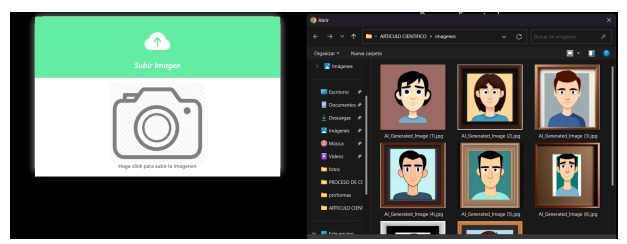
\includegraphics[width=0.7\linewidth]{figura 3.jpeg}
    \caption{Carga de imágenes en la aplicación}
    \label{fig:enter-label}
\end{figure}
\begin{figure}
    \centering
    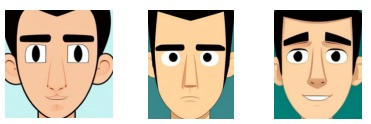
\includegraphics[width=0.7\linewidth]{figura 2.jpeg}
    \caption{Recorte de rasgos faciales}
    \label{fig:enter-label}
\end{figure}

\subsection{Microservicios}
Microservicios son modulares autónomos que operan con independencia y mantengan una comunicación coherente a través de una interfaz estandarizada y compartida. Se especifican cada microservicio como guardar persona, reconocer, recorte facial, borrar contenido, y registrar el rostro. Se enfoca en el registro de individuos, compartir en evaluación, identificar rostros en la imagen, y eliminar contenido para evitar la acumulación innecesaria de información.
\\El microservicio web proporciona un tiempo de respuesta rápido, lo que permite la detección de rostros en tiempo real.
El sistema de detección de rostros presenta una precisión alta, con un bajo índice de falsos positivos y falsos negativos.
La arquitectura basada en microservicios permite escalar el sistema fácilmente para manejar un gran volumen de peticiones.
\begin{itemize}
    \item El sistema en la detección facial es capaz de guardar personas en casos de que un individuo no está registrado en la base de datos.
    \item Reconocer el rostro: Compara las codificaciones faciales almacenadas y actuales en evaluación, ejecutar una correspondencia y initiar el proceso de reconocimiento.
    \item Recorte facial: produce una nueva imagen centrada en el rostro detectado, y extrayendo características específicas a través de encodings.
    \item Eliminar Contenido: Para prevenir la acumulación innecesaria de datos tras la carga de la imagen en el sistema, se lleva a cabo una operación de supresión del contenido pertinente.
    \item Servicio de almacenamiento.
\end{itemize}

\begin{figure}[ht]
  \centering
  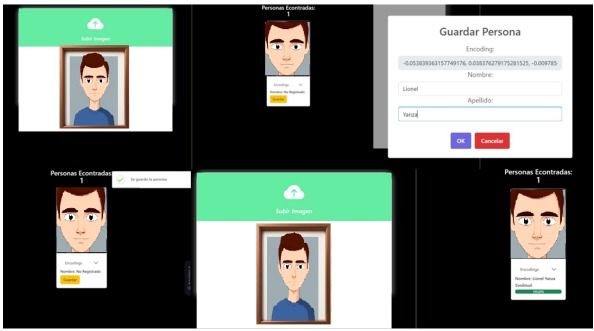
\includegraphics[width=0.7\textwidth]{figura1.jpeg}
  \caption{Registro de una nueva identidad}
\end{figure}

\section{Resultados}
Al principio de la investigación, se seleccionaron 20 imágenes JPG y PNG para evaluar la eficacia de un microservicio desarrollado. Estas imágenes se cargaron en el sistema para comenzar a procesar imágenes faciales. El sistema luego avanzó hacia la identificación de rostros mediante algoritmos específicos, y las imágenes se guardaron en una carpeta en el fondo.
\\La precisión del sistema de detección de rostros es alta y el tiempo de respuesta es rápido. La arquitectura basada en microservicios permite escalar el sistema fácilmente para manejar un gran volumen de peticiones. Sin embargo, la precisión del sistema puede verse afectada por la calidad de las imágenes, la iluminación y el ángulo de la cámara.

\section{Discusión y conclusiones}
El microservicio web para la detección de rostros es un recurso poderoso en el reconocimiento facial. Su arquitectura basada en microservicios ofrece una modularidad y escalabilidad, permitiendo más eficiente implementación y mantenimiento. La gestión de datos se optimiza mediante análisis de similitud coseno en las representaciones faciales almacenadas, y la incorporación de tecnologías de aprendizaje profundo.
\\
Este proyecto ha desarrollado un microservicio web efectivo para la detección de rostros utilizando FaceNet-PyTorch. Los resultados obtenidos demuestran la precisión y la eficiencia del sistema. Para trabajos futuros, se podrían explorar otras técnicas de aprendizaje profundo para mejorar la precisión del sistema. Además, se podrían integrar otras funcionalidades al microservicio, como la identificación de emociones o el reconocimiento de rostros.

\section{Referências}
{\begin{enumerate}
    \item Yanza-Saca, G. X., Tenesaca-Pesántez, J. A. (2023). Microservicio web para la detección de rostros. MQRInvestigar, 7(3), 4018–4034. https://doi.org/10.56048/mqr20225.7.3.2023.4018-4034.
    \item M. J. Gonçalves, hiberus blog, hiberus blog, 13 Octubre 2021. Available:
    https://www.hiberus.com/crecemos-contigo/que-es-angular-y-para-que-sirve/. [Último acceso:
    14 Agosto 2023].
    \item rockcontent blog, rockcontent blog, 12 Abril 2020. [En línea]. Available:
    https://rockcontent.com/es/blog/bootstrap/. [Último acceso: 14 Agosto 2023].
    \item estrada web group,estrada web group, En línea. Available:
    https://estradawebgroup.com/Post/Mensajes-de-notificacion-profesionales-al-usuario-conjQuery-y-SweetAlert/4252?expand-article=1. [Último acceso: 14 Agosto 2023].
    \item D. E. Espinoza Olguín y P. I. Jorquera Guillen , Reconocimiento Facial, PONTIFICIA UNIVERSIDAD CATÓLICA DE VALPARAÍSO FACULTAD DE INGENIERÍA ESCUELA DE INGENIERÍA INFORMÁTICA , Valparaiso, 2015
    \item M. Andrejevic y N. Selwyn, Facial recognition technology in schools: critical questions andconcerns, Taylor y Francis Online, 2019.
    
    \item K T. Gómez Suárez, R. Anaya y A. F. Cano, Un acercamiento a los microservicios,UNACIENCIA, 2017.
    \item R. M. Barreto Rodriguez y D. J. Lizarraga Mendoza , Modelo de Sistema de Reconocimiento Facial para el Control de la Trata de Personas”, Universidad Tecnologica del Peru, Arequipa, 2019.
    \item A. M. Sichique Pillacela y M. E. Guerrero Zhunio, Diseño y desarrollo de un sistema de prototipo de reconocimiento facial sobre infraestructura Fog Computing en una arquitectura de microservicios montada en contenedores Docker ejecutadas en una instancia de infraestructura de nube distribuida en OpenNebu, Universidad Politecnica Salesiana, Cuenca,202.

    \item J. C. Ortega Castro, A. S. Quevedo Sacoto, G. V. Saltos Bernal y J. F. Illescas Peña,Educación digital, blockchain y su influencia sobre la economía popular y solidaria,Conrado, 2023.
    \item P. Quevedo Avila, M. G. Zhindón Mora y A. S. Quevedo Sacoto, Arquitectura de microservicios para compras en línea: caso de uso" ala orden", Imprenta y Casa Editora" Coni", 2020.
    \item  A. F. Ruiz Velasco y S. M. Roa Martínez, Arquitectura de microservicios para extracción, 2020.
    
\end{enumerate}}
\end{document}
